\chapter{Proceso de negocio. Fundamentos teóricos}
\label{chap:teoria}

\lettrine{A} { día} de hoy es innegable el papel crucial que juegan las tecnologías de la información en general y los sistemas de información en particular dentro de la gestión de procesos de negocio de cara a la consecución de objetivos de forma eficaz y eficiente. 

El mercado está en continua evolución. Los sistemas de información nos proporcionan la tecnología básica necesaria tanto para crear nuevas funcionalidades como para adaptar las existentes para poder satisfacer las nuevas necesidades que van surgiendo. 

Este capítulo pretende ser una aproximación a los conceptos teóricos en los que se enmarcan los procesos empresariales dentro del sector \acrfull{tic}.


\section{Proceso de negocio}

Hammer \& Champy (1993)~\cite{Hammer-Champy} definieron el proceso de negocio como:

\begin{displayquote}
Una colección de actividades que toman uno o más tipos de entradas y crean una salida que tiene valor para el cliente. 
\end{displayquote}

Así pues, podemos entender un proceso de negocio como un conjunto de funciones dentro de una secuencia específica que proporciona valor a un cliente interno o externo y cada función dentro de un proceso puede ser a su vez interpretado como un proceso en si mismo llamado sub-proceso. El desencadenante de este subproceso es el proceso previo (o por el evento inicial que da comienzo al proceso en general) y devuelve un resultado de valor para el siguiente proceso o para el cliente final y sus procesos si este es el último suproceso de un proceso de extremo a extremo~\cite{Kirchmer}. 

Esta descomposición de procesos en subprocesos puede extenderse tanto como las funciones resultados sigan teniendo sentido desde el punto de vista de negocio: por ejemplo el subproceso "gestión de ventas" puede describirse en detalle usando funciones como "registro de orden de venta" o "asignación de productos a la orden de venta", sin embargo descomponer la función "registro de orden de venta" en actividades como "introducir nombre de cliente", "introducir dirección de cliente", etc. no aportan relevancia alguna desde el punto de vista de negocio.

Con el objetivo de poder definir de forma sencilla los procesos más complejos sin dejar de lado ningún aspecto importante de los mismos surge la \acrfull{aris}, una aproximación al proceso de arquitectura y modelado empresarial desarrlollado por August-Wilhem Scheers y que permite describir un proceso de negocio desde cinco puntos de vista diferentes, dando respuesta a todas las cuestiones relevantes relativas al proceso:

\begin{itemize}
\item Vista organizacional: ¿quién (gente, departamentos, empresas, etc.) está involucrado en el proceso?
\item Vista funcional: ¿qué funciones se llevan a cabo dentro del proceso?
\item Vista de datos: ¿qué datos o información es necesaria/producida para/en el proceso?
\item Vista de entrega: ¿qué son los entregables del proceso y por qué los necesito?
\item Vista de control: el cómo se ve en conjunto refleja el quién está haciendo qué, qué datos producen entregables y cual es la secuencia lógica que hace que las funciones lleven a cabo su función.
\end{itemize}


La figura ~\ref{fig:aris} (página~\pageref{fig:aris})  muestra la arquitectura \acrshort{aris}:


\begin{figure}[H]
  \centering
  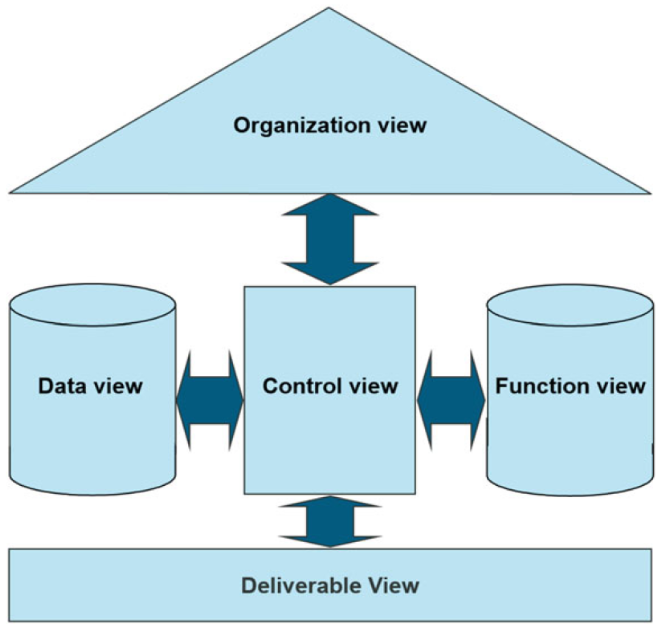
\includegraphics[width=0.30\textwidth]{imaxes/aris.png}
  \caption{Arquitectura de sistema de información integrada (\acrshort{aris})}
  \label{fig:aris}
\end{figure}


El elemento más importante de la arquitectura \acrshort{aris} es la vista de control. Esta muestra como dos o más aspectos de un proceso \textit{encajan}, por ejemplo quién es responsable de una función determinada o qué función usa determinados datos. La vista resultado de la integración de varios aspectos del proceso de negocio es la llave para la gestión exitosa de dichos procesos. \acrshort{aris} ayuda a convertir los procesos en algo \textit{tangible} al definir cómo describirlos asentando la base para convertir la \acrlong{bpm} en una disciplina de gestión real.


\subsection{Gestión de proceso de negocio}

Un \acrfull{bpm} incluye conceptos, métodos y tecnicas para soportar el diseño, la administración, la configuración, la representación y el análisis de los procesos de negocio~\cite{Weske}.

La base del \acrshort{bpm} es la representación explícita de los procesos de negocio con sus actividades y las restricciones de ejecución de los mismos.


El ciclo de vida del \acrshort{bpm} consta de cinco fases~\cite{bpmLifecycle} tal y como se muestra en la figura ~\ref{fig:lifecycle-bpm} (página~\pageref{fig:lifecycle-bpm}):


\begin{figure}[hp!]
  \centering
  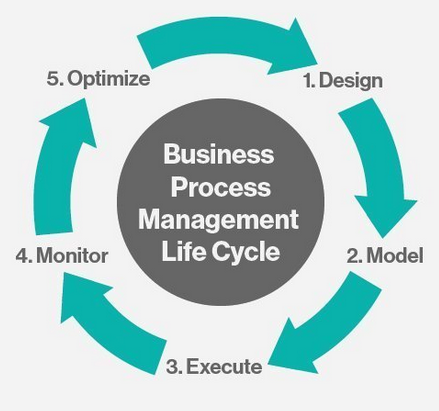
\includegraphics[width=0.30\textwidth]{imaxes/bpm-lifecycle.png}
  \caption{Ciclo de vida del \acrshort{bpm}}
  \label{fig:lifecycle-bpm}
\end{figure}

\begin{enumerate}
\item Diseño: el diseño de procesos abarca tanto la identificación de procesos existentes como el diseño de procesos "futuros". El objetivo de este paso es garantizar un diseño correcto y eficiente. Debe haber una sincronización entre los procesos existentes y el diseño de un nuevo proceso para evitar posibles interrupciones.
\item Modelado: se crea una representación visual del modelo de proceso. Esto debe incluir detalles específicos, como líneas de tiempo, descripciones de tareas y cualquier flujo de datos en el proceso. 
\item Ejecución: consiste en una prueba de concepto, probando el nuevo sistema BPM con un grupo limitado. Después de incorporar cualquier comentario, el equipo puede comenzar a implementar el proceso a un público más amplio.
\item Supervisión:  durante esta etapa, se supervisa el proceso, se miden las mejoras en la eficiencia y se identifica cualquier cuello de botella adicional.
\item Optimización: se realizan los ajustes finales al proceso para mejorar la actividad empresarial.

\end{enumerate}

Entre las ventajas que proporcionan los \acrshort{bpm} se encuentran las siguientes:

\begin{itemize}
\item Mayor eficiencia y ahorro de costes: gracias a la optimización de los procesos existentes y a la incorporación de más estructura en el desarrollo de nuevos procesos, eliminando redundancias y cuellos de botella.
\item Mejor experiencia de empleados y clientes: ya que permite eliminar el trabajo repetitivo y aumentar la accesibilidad de la información mejorando la productividad y la implicación con el cliente.
\item Procesos más escalables: a través de la mejora en la ejecución de procesos y la automatización de flujos de trabajo se facilita el escalado de procesos a otras zonas geográficas de todo el mundo.
\item Mayor transparencia: puesto que la automatización de procesos de negocio define claramente a los propietarios para las tareas a lo largo del proceso, se proporciona más transparencia y responsabilidad a lo largo de un proceso determinad, favoreciendo la comunicación entre equipos.
\end{itemize}




\section{Sistemas de soporte operacional y Sistemas de soporte de negocio}

Centrándonos en el área de las telecomunicaciones, nos encontramos con dos nuevos conceptos:


\acrfull{oss}. Se trata de un término usado para describir los sistemas de procesado de información utilizados por las operadoras para gestionar sus redes de comunicación. Originalmente conocidas como herramientas de Gestión de redes de telecomunicaciones o Telecommunication Network Management tools actualmente estas soluciones son mucho más sofisticadas, permitiendo coordinar clientes, servicios, recursos, procesos y actividades. Ayudan a las operadoras a diseñar, construir, operar y mantener las redes de comunicaciones.

\acrfull{bss} es el término tradicionalmente utilizado para describir las funcionalidades de negocio y/o orientada al cliente. Estas herramientas  permiten que una organización contacte con sus clientes (por ejemplo a través del \acrshort{crm}), crear ofertas para ellos, emitir facturas así como transacciones entre operadores de comunicaciones (liquidaciones, punto de interconexión).

De forma conjunta \acrshort{oss} y \acrshort{bss} permiten a los operadores de red ofrecer servicios de manera eficiente y confiable a un enorme número de suscriptores en algunas de las máquinas más complejas del mundo, las redes globales de telecomunicaciones.

Existen distintos estándares para aportar consistencia entre las distintas aplicaciones existentes. Comentaremos brevemente algunas de ellas.

\subsection{TMN de ITU-T}

Las Comisiones de Estudio del \acrfull{itut} reúnen a expertos de todo el mundo para elaborar documentos de especificación de telecomunicaciones y protocolos informáticos, conocidos como Recomendaciones ITU-T, que actúan como elementos definitorios de la infraestructura mundial de las \acrfull{tic}  ~\cite{ITU-T}. 

Los esfuerzos de normalización de la \acrshort{itut} comenzaron en 1865 con la formación de la International Telegraph Union (en español Unión Telegráfica Internacional), que más tarde se convirtió en la \acrfull{itu}. La \acrshort{itu} se convirtió en un organismo especializado de las Naciones Unidas en 1947. El \acrfull{ccitt} fue creado en 1956, y pasó a llamarse \acrshort{itut} en 1993.


El modelo tecnológico \acrshort{tmn} se presenta en la recomendación M.3010 y suele referenciarse como la pirámide \acrshort{tmn} (figura ~\ref{fig:pirámide-tmn}, página~\pageref{fig:pirámide-tmn}). Aborda la complejidad de la gestión de las telecomunicaciones a través de una arquitectura lógica por capas, la cual organiza las funciones en grupos denominados capas lógicas y describe las relaciones entre las mismas. Una capa lógica refleja aspectos particulares de la gestión e implica el agrupamiento de la información de gestión relativa a ese aspecto. Estas capas son las siguientes:

\begin{itemize}
\item Capa de gestión de elementos. Proporciona definición y coordinación de una colección de dispositivos de red, aunque sea un subconjunto de toda la red. Esta capa normalmente incluiría la consolidación de la administración de alarmas, la copia de seguridad, el registro y el mantenimiento de los sistemas que admiten los dispositivos de red.
\item Capa de gestión de red. Proporciona la vista de administración general de la red como una suma de partes componentes. Es responsable de la supervisión, configuración y control de extremo a extremo de la red.
\item Capa de gestión de servicios. Responsable de definir los servicios ofrecidos por las operadoras de comunicaciones. Esto proporciona la interfaz entre los servicios de un cliente y la red, incluyendo la definición, la administración y la carga.
\item Capa de gestión empresarial. Representa la funcionalidad relacionada con la planificación estratégica del negocio, como las tendencias, la calidad, etc., y proporciona la base para la facturación, el presupuesto y el establecimiento de objetivos.
\end{itemize}


\begin{figure}[H]
  \centering
  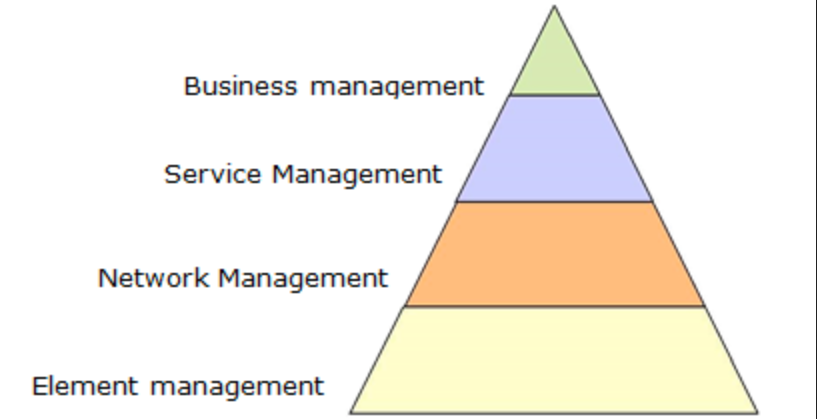
\includegraphics[width=0.40\textwidth]{imaxes/piramide-tmn.png}
  \caption{Modelo tecnológico \acrshort{tmn}}
  \label{fig:pirámide-tmn}
\end{figure}


Las áreas funcionales de gestión presentadas en la recomendación M.3400 incluyen entre otras las siguientes áreas: 
\begin{enumerate}
\item Administración de clientes.
\item Gestión de aprovisionamiento de red.
\item Administración de tarifas, cobros y contabilidad.
\item Administración de Medición y Análisis de Tráfico
\item Gestión del tráfico.
\item Administración de Enrutamiento y Análisis de Dígitos
\item Administración de Seguridad.
\end{enumerate}


\subsection{TMF}

\acrlong{tmf} es una alianza compuesta por más de 850 compañías globales que trabajan conjuntamente proporcionando un entorno abierto y colaborativo y un soporte práctico que permite a las compañías proveedoras de servicios y sus distribuidores transformar rápidamente sus operaciones comerciales, sistemas de TI y ecosistemas para capitalizar las oportunidades presentadas en un mundo digital en rápida evolución~\cite{TMFORUM}.

\acrshort{tmf} fue fundada como OSI/Network Management Forum (en español Foro de Gestión de Redes/OSI) en 1988 por ocho empresas para resolver de forma conjunta los problemas de gestión operativa y de sistemas con los protocolos OSI. En 1998 el nombre fue cambiado a TeleManagement Forum. En 2008, la organización cambió su nombre a TM Forum.

A través de estas colaboraciones los modelos de \acrshort{tmn} han ganado un uso generalizado en el campo de las implementaciones de OSS. Dentro de los trabajos desarrollados por el \acrshort{tmf} encuentra el Frameworx. Se trata un marco de arquitectura empresarial orientado a los proveedores de servicios de comunicaciones que consta de 4 marcos de trabajo o frameworks:

\begin{enumerate}
\item Un modelo de aplicación (\acrfull{tam}). Proporciona un marco modular de bloques funcionales de gestión. Esto ayuda a proporcionar una mayor consistencia (y compatibilidad) entre los conjuntos de productos de diferentes proveedores (figura ~\ref{fig:tam}, página~\pageref{fig:tam}).
\item Un modelo de proceso (\acrfull{etom}). Tiene como objetivo proporcionar un lenguaje común y un catálogo de procesos de negocio utilizados en entornos de telecomunicaciones. Este nivel de normalización tiene por objeto simplificar las líneas de comunicación entre los proveedores de servicios y los integradores de sistemas asociados (figura ~\ref{fig:etom}, página~\pageref{fig:etom}).
\item Un modelo de información (\acrfull{sid}). Su objetivo es definir las entidades esenciales, las relaciones y los atributos de los objetos de datos que prevalecen en las aplicaciones/bases de datos de telecomunicaciones. También proporciona un lenguaje común para su uso por los desarrolladores/integradores de OSS. (\acrshort{tmf}) también ha tratado de desarrollar API estandarizadas basadas en SID (interfaces de programación de aplicaciones) como OSS/J para acelerar la integración de sistemas dispares.
\item Un marco de integración de sistemas (\acrfull{tna}). Tiene como objetivo proporcionar estandarización arquitectónica, sin dejar de ser tecnológicamente neutral, incluyendo interfaces, mecanismos y políticas comunes. La integración también se conoce comúnmente como el (\acrfull{tip})
\end{enumerate}

\begin{figure}[H]
  \centering
  \begin{subfigure}[c]{0.3\textwidth}
    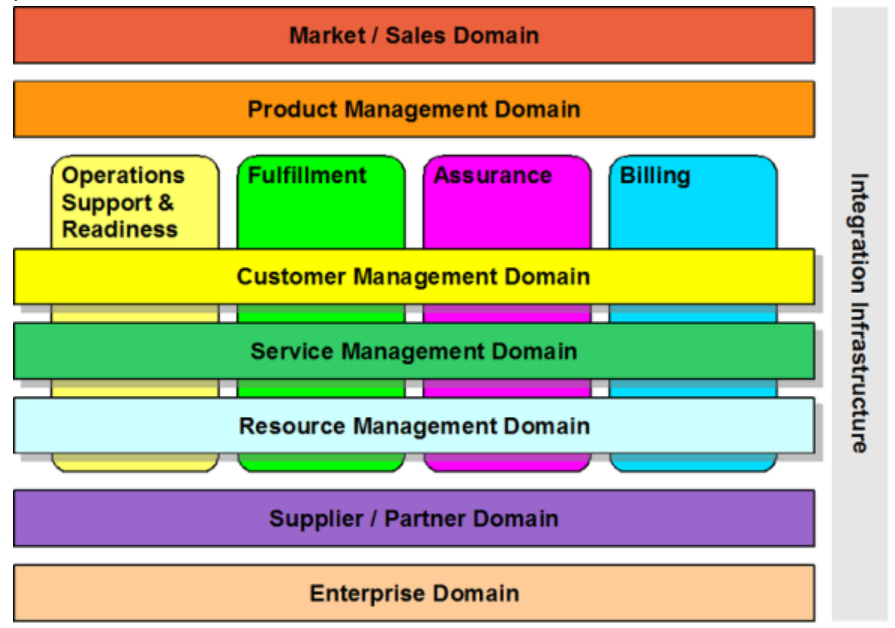
\includegraphics[width=\textwidth]{imaxes/tam.png}
    \caption{Modelo de proceso \acrshort{tam}}
    \label{fig:tam}
  \end{subfigure}
  \hspace{0.1\textwidth}
  \begin{subfigure}[c]{0.3\textwidth}
    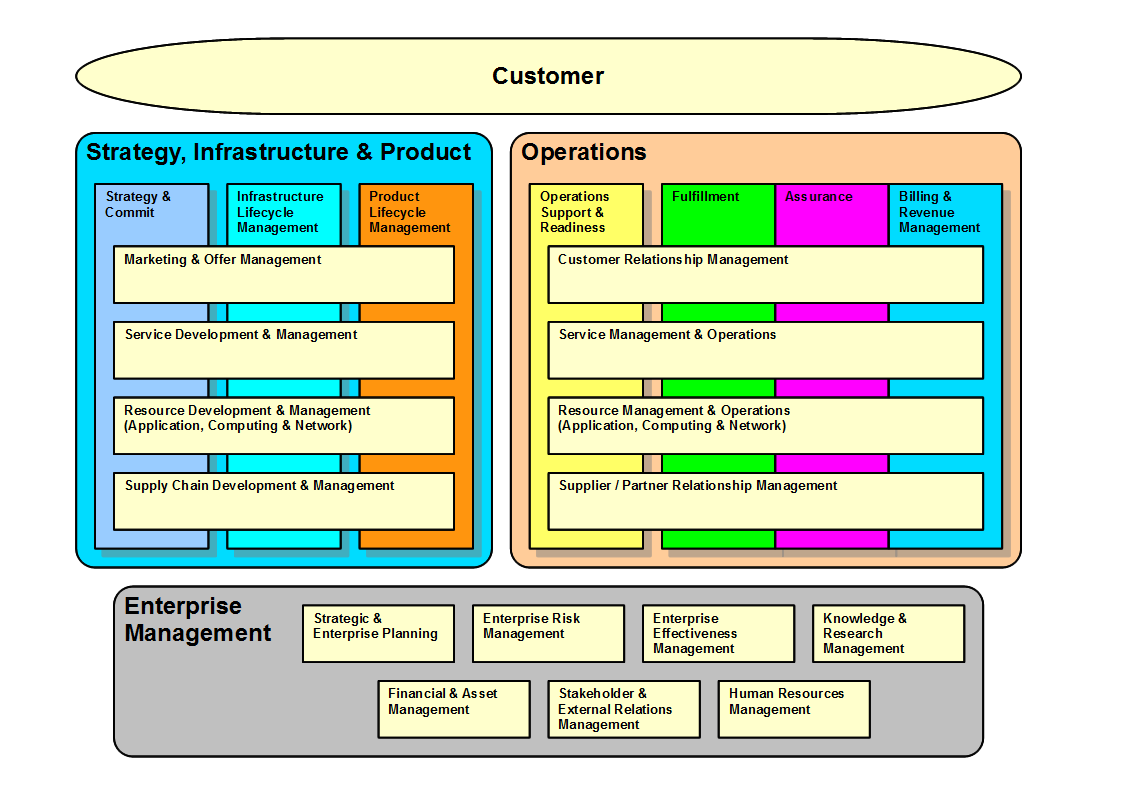
\includegraphics[width=\textwidth,height=3cm]{imaxes/etom.png}
    \caption{Modelo de proceso \acrshort{etom}}
    \label{fig:etom}
  \end{subfigure}
  \caption{Modelos de referencia del marco de trabajo de \acrshort{tmn}}
  \label{fig:tam-etom}
\end{figure}


Además de estos marcos de trabajo (\acrshort{tmf}), el (\acrlong{tmf}) cuenta con la suite TM Forum Open API, que tiene más de 50 API basadas en REST (y muchas más en desarrollo) y con un el (\acrfull{oda}), un estándar en evolución que tiene la intención de establecer una nueva visión para \acrshort{oss}/\acrshort{bss} que parecen estar ganando uso generalizado en el mundo de las telecomunicaciones.


\subsection{ITIL e ITSM}

\acrfull{itil} describe procesos, procedimientos, tareas y listas de verificación que no son ni específicos de la organización ni de la tecnología, pero que pueden ser aplicados por una organización hacia la estrategia, la entrega de valor y el mantenimiento de un nivel mínimo de competencia. Se creó originalmente en la década de 1980 como una colección de libros, cada uno de los cuales cubría una práctica específica de gestión de servicios de \acrshort{ti}. Fue desarrollado por el Gobierno del Reino Unido en un intento de estandarizar los procesos de \acrshort{ti}, en particular el traspaso de la implementación a los entornos de soporte de \acrshort{ti} en curso. Entre 1986 y 1996, esta colección aumentó a más de 30 volúmenes. Durante los años 2000 y 2001 estos volúmenes se consolidaron en 9 conjuntos que agrupaban temas relacionados~\cite{Exin, ItilWiki}. 


\acrfull{itsm} es un conjunto de políticas, procesos y procedimientos para gestionar la implementación, mejora y soporte de servicios de \acrshort{ti} orientados al cliente. A diferencia de otras prácticas de gestión de \acrshort{ti} que se centran en hardware, redes o sistemas, \acrshort{itsm} es un enfoque más centrado en los procesos y las personas, teniendo como objetivo la mejora constante el servicio al cliente de \acrshort{ti} de forma alineada a los objetivos comerciales. Las empresas que utilizan \acrshort{itsm} consideran la \acrshort{ti} como un servicio, con un enfoque en la prestación de servicios valiosos a los clientes, en lugar de un departamento que administra la tecnología.

Los principales elementos de \acrshort{itsm} son:

\begin{itemize}
\item Gestión de incidencias.
\item Gestión de problemas. 
\item Gestión del cambio. 
\item Gestión de proyectos. 
\item Gestión de activos. 
\item Conocimiento, política y procedimiento. 
\item Catálogo de servicios. 
\item \textit{Service Desk.}
\end{itemize}

Aunque a veces se usan indistintamente, \acrshort{itsm} e \acrshort{itil} no son lo mismo: \acrshort{itil} es uno de los marcos más populares dentro de la disciplina \acrshort{itsm}, y ha ayudado a informar e inspirar otros marcos \acrshort{itsm}. Por lo tanto \acrshort{itil} es la base en la que se apoya \acrshort{itsm} proporcionando a las empresas la metodología necesaria para adoptar e implementar \acrshort{itsm} (figura ~\ref{fig:itil-vs-itsm},  página~\pageref{fig:itil-vs-itsm})

\begin{figure}[H]
  \centering
  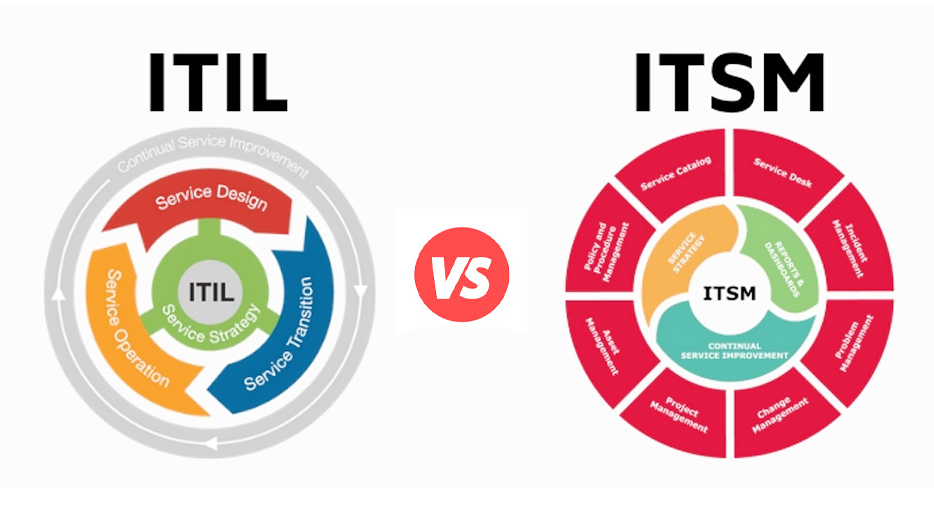
\includegraphics[width=0.30\textwidth]{imaxes/itil-vs-itsm.png}
  \caption{ \acrshort{itil} y \acrshort{itsm}}
  \label{fig:itil-vs-itsm}
\end{figure}



Por otro lado, de la misma forma que existe una una superposición cada vez mayor entre las \acrshort{ti} y las tecnologías de redes de telecomunicaciones, también hay una mayor prevalencia de marcos de \acrshort{ti} (como \acrshort{itil}) que se utilizan junto con los marcos de telecomunicaciones (como \acrshort{etom}). Los proveedores de servicios de telecomunicaciones dependen de una infraestructura de TI altamente confiable (por ejemplo, servidores, etc.) e ITIL se considera actualmente como la mejor práctica para la gestión de este tipo de activos. Del mismo modo, los clientes están subcontratando la gestión de la infraestructura de TI y telecomunicaciones de extremo a extremo, exigiendo a sus proveedores de servicios que suministren una gestión de servicios de alta calidad de la red y los activos de TI cada vez más críticos del cliente.


\acrshort{etom} comparte algunos puntos en común y varias diferencias con \acrshort{itil}. \acrshort{tmf} ha publicado una nota de aplicación eTOM – ITIL (GB921L) titulada "Using eTOM to model the ITIL Processes". Esta nota proporciona orientación sobre el modelado de la gestión de servicios de \acrshort{ti} utilizando los elementos de proceso estándar dentro de \acrshort{etom} así como una superposición detallada de procesos \acrshort{itil} con procesos \acrshort{etom} (figura ~\ref{fig:itil-etom}, página~\pageref{fig:itil-etom})



\begin{figure}[H]
  \centering
  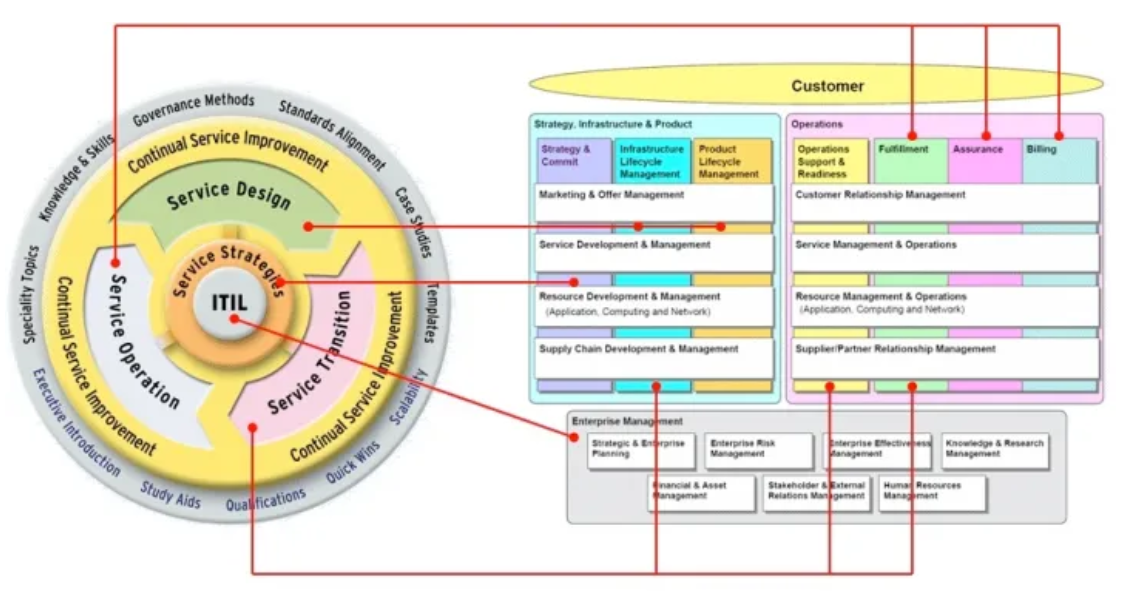
\includegraphics[width=0.30\textwidth]{imaxes/etom-itil.png}
  \caption{Aproximación al mapeo entre \acrshort{etom} e \acrshort{itil}~\cite{Itil-eTom}}
  \label{fig:itil-etom}
\end{figure}


\section{Gestión de relaciones con los clientes}


La \acrfull{crm} es una estrategia comercial que optimiza los ingresos y la rentabilidad al tiempo que promueve la satisfacción y la lealtad del cliente. Las tecnologías CRM permiten la estrategia, e identifican y gestionan las relaciones con los clientes~\cite{GartnerCRM}. El compendio de conceptos, procedimientos y reglas que una corporación sigue al comunicarse con sus consumidores se conocen como  \acrshort{crm}~\cite{WikiCRM} y por definición cubre todas las formas en las que se administran las relaciones con los clientes en los distintos ámbitos empresariales: ventas, marketing, servicio al cliente y comercio electrónico~\cite{SAP-CRM} . 

Por lo general, cuando hablamos de \acrshort{crm} estamos refiriéndonos a los sistemas de software que nos ayudan a construir estrategias de negocio para retener y captar clientes.
El software \acrfull{crm} permite automatizar e integrar estas actividades orientadas al cliente e incluso pueden ofrecer herramientas para el análisis de clientes, la personalización, las redes sociales, la colaboración y mucho más. La funcionalidad que el software \acrshort{crm} proporciona a las empresas se divide en cuatro segmentos: ventas, marketing, servicio al clientes y comercio digital~\cite{GartnerCRM}. 


\subsection{Breve historia del CRM}

La necesidad de mantener registros relativos a la información comercial no es algo nuevo. De hecho podríamos decir que existe desde que existe el comercio: con el tiempo el saber quien poseía qué o quien debía a quién requiería alguna forma de notación y registro permanente, así como alguna forma de contabilidad para la gestión de los bienes. El tratamiento de esta información fue evolucionando adaptándose a las necesidades que iban surgiendo en cada momento como pudiera ser la segmentación de clientes atendiendo a sus capacidad de pago o a su nivel económico, permitiendo aplicar distintas estrategias comerciales en función de la información almacenada. 


La aparición del Rodolex (palabra compuesta a partir de las palabras \textit{rolling} e \textit{index}) en la década de los 50 (figura ~\ref{fig:rodolex} , página~\pageref{fig:rodolex}) supuso un gran avance en el tratamiento de los clientes. Este dispositivo giratorio que permitía almacenar tarjetas indexadas de quita y pon que contenían la información relevante de distintas personas y empresas, resultó ser una forma mucho más rápida, cómoda y eficaz de acceder y/o modificar dicha información que los métodos existentes hasta el momento (principalmente la búsqueda de información en libros de contabilidad y archivos personales del cliente). Este término se ha vuelto algo genérico para nombrar cualquier organizador personal que realice esta función, o como una metonimia para el total de los contactos comerciales acumulados de un individuo.


\begin{figure}[H]
  \centering
  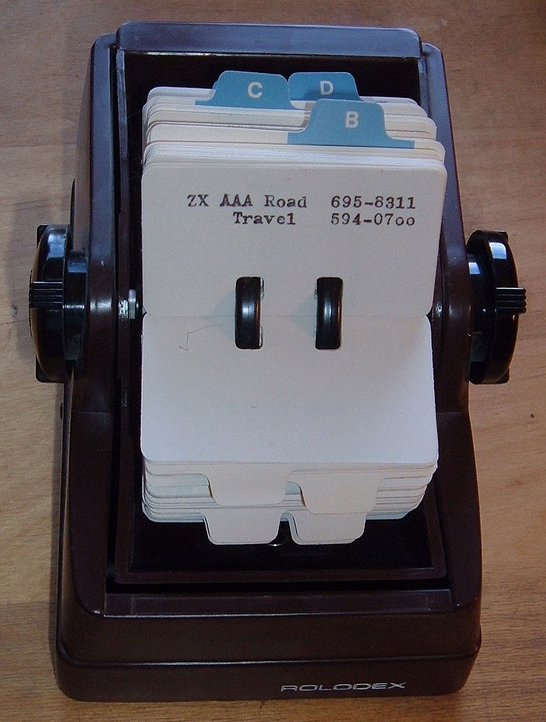
\includegraphics[width=0.3\textwidth]{imaxes/rodolex.png}
  \caption{Rodolex}
  \label{fig:rodolex}
\end{figure}




En la década de los 60 comienza la introducción de las computadoras en las empresas. Los sistemas de mainframe independientes se hicieron ampliamente disponibles para las empresas lo que les permitiría manejar bases de datos de los clientes y aplicar un nivel (básico) de automatización, ayudando a mantener registros contables. Inicialmente la gestión de clientes pertenecía al departamento de cuentas, pero esta automatización pronto se extendió a otros departamentos, incluidos ventas y marketing. En la década de los 70 el precio de los ordenadores disminuyó drásticamente, lo que permitió que hasta las pequeñas empresas se sumaran al carro de la revolución informática y a partir de ahí vino la siguiente evolución del CRM.


Los inicios del CRM tal como lo conocemos comenzaron en la década de 1980. En esta época se produzco el cámbio del márketing directo al márketing de base de datos. Esto marca el comienzo de la combinación de datos de clientes con estrategia de ventas, una parte central de CRM tal como lo conocemos hoy~\citep{ThinkautomationCRM}:

\begin{itemize}
\item Marketing directo: Cualquier práctica de marketing que implique comunicación directa o interacción con clientes individuales. Por ejemplo, a través de la comunicación postal directa como catálogos y cartas.
\item Marketing de base de datos: Una forma de marketing directo que implica recopilar datos de clientes, analizar estos datos y usarlos para crear mensajes de marketing personalizados y predecir las acciones y deseos de nuevos clientes potenciales. Se trata de utilizar datos para optimizar los esfuerzos de marketing.
\end{itemize}


Robert y Kate Kestnbaum fueron pioneros del marketing de bases de datos. Se trataba de una forma de marketing directo que analizaba estadísticamente la base de datos de clientes para identificar qué clientes tendrían más probabilidades de reaccionar a una campaña de marketing. El concepto despegó y Kestnbaum, junto con Robert Shaw, nos trajo nuevos conceptos y metodologías, que van desde el valor de por vida del cliente hasta la gestión del canal. En 1986, Pat Sullivan y Mike Muhney lanzaron un sistema de evaluación de clientes llamado ACT! (acrónimo de "Automated Contact Tracking" - Seguimiento automatizado de contactos en español) basado en el principio de Rolodex digital, que ofrecía por primera vez un servicio de gestión de contactos que facilitaba el almacenamiento de información de contactos (nombres, direcciones, números de teléfono, etc.), lo que podría considerarse como el primer CRM automatizado~\cite{SalesforceCRM}. 


A medida que las oficinas se digitalizaron a lo largo de la década de 1990 surgieron una gran cantidad de nuevos productos de gestión de datos de clientes. Estos productos se definían como \acrfull{sfa} y eran una amalgama de márketing de base de datos y gestión de contactos. En 1993, Tom Siebel diseñó el primer producto de \acrshort{crm}, Siebel Customer Relationship Management. Con el fin de competir con estas novedosas soluciones de \acrshort{crm}, las empresas de \acrfull{erp}\footnote{\acrshort{erp}: sofware que se ocupa de la gestión de los principales procesos comerciales, incluidas las áreas relacionadas con las relaciones con los clientes} también vieron una oportunidad y el mercado se volvió muy competitivo. A mediados de los años 90, este mercado se disparó en ofertas de productos de todas las formas y tamaños, ahora conocidas como sistemas \acrshort{crm}. La gestión de relaciones con los clientes se popularizó en 1997, debido al trabajo de Siebel, Gartner e IBM. Entre 1997 y 2000, los principales productos de \acrshort{crm}. se enriquecieron con capacidades de envío y marketing. Siebel introdujo la primera aplicación de \acrshort{crm}. móvil llamada Siebel Sales Handheld en 1999. La idea de una base de clientes independiente y alojada en la nube pronto fue adoptada por otros proveedores líderes en ese momento, incluidos PeopleSoft (adquirido por Oracle), Oracle, SAP y Salesforce.com.

Y así llegamos a nuestros días, en los que el mercado de nuevos productos \acrshort{crm} no parece haber alcanzado su punto de saturación. Las nuevas empresas continúan llegando al mercado con productos en la nube, mientras que los proveedores existentes han cambiado sus modelos de licencia para ofrecer alternativas en la nube a las licencias de sitios tradicionales. El último cambio es el aumento de los datos sociales y la necesidad de interactuar con los clientes en las diversas plataformas sociales. El móvil se ha vuelto aún más imperativo como una oferta con la llegada del teléfono inteligente. El ritmo del cambio es tan rápido que muchos proveedores están luchando para mantenerse al tanto de los últimos desarrollos, que van desde chatbots hasta big data e IA. Si bien se podría esperar que los productos de \acrshort{crm} hayan madurado, los clientes aún experimentan dificultades para lograr implementaciones exitosas. Esto se debe a que ellos también están luchando por mantener sus modelos de negocio relevantes y sostenibles en esta era disruptiva.
